\subsection{Disparity Testing}
After verifying that the camera interface was functional, a large portion of time was spent implementing a disparity algorithm that would allow for the extraction of 3D depth information from stereo image data. This algorithm was first implemented in \textsc{Matlab}, and was then transferred to programmable logic after the algorithm was verified working. 

\subsubsection{Image Rectification}
In order to perform the most accurate block matching as possible on camera image data, it would be ideal to rectify the images as outlined in Section \ref{rectsec}. However, since the image data used in the disparity calculation contains a central 384x288 image taken from the middle of each 752x480 input image, a large portion of the input image is cropped out. Since many of the lens artifacts corrected using a rectification process are contained on the external edges of the input imagery, no additional camera calibration is performed in the disparity or camera controller implementations \cite{collins}. 
\par
After extensive testing with the stereo camera breakout board and disparity module detailed in the following sections, it was also found that the camera imagery captured through the stereo camera interface contains consistent horizontal epipolar lines between both images. These lines are accurate enough for the custom disparity algorithm to process without additional calibration, saving a large amount of calibration time in the image processing pipeline. Along with the aforementioned reasons, a full camera calibration and image rectification process was not implemented in FPGA hardware due to time constraints, although a cursory calibration process was examined in \textsc{Matlab}. With the issue of camera calibration and image rectification addressed, it was then possible to begin implementing a test disparity algorithm in \textsc{Matlab}.

\subsubsection{\textsc{Matlab} Implementation}
The Sum of Absolute Differences algorithm discussed in Section \ref{SADexample} was implemented first implemented using \textsc{Matlab}, and can be found in Appendix item \ref{disparityTestMatlab} \cite{mccormick}. This implementation has been created to operate on the "cones" standard test image set, and produces a resultant disparity image from its given input images. In the case of this specific example, the algorithm performs a 7x7 Sum of Absolute Differences block matching process on 50 search ranges of horizontal epipolar lines between the two images. However, the block size and search range may be customized by the user to test the functionality of the algorithm. 
\par
Overall, the \textsc{Matlab} disparity test implementation may be broken down into the following steps:
\par
\singlespacing
\begin{enumerate}
\item
Load in image data (also convert to grayscale if using the "cones" image set)
\item
Determine the size of the template image and create a resultant matrix to store output disparity values in
\item
For each full row of pixels across an image, perform the following steps:
\begin{enumerate}
\item
Set minimum and maximum row bounds for the current block of pixels being used for SAD 
\item
For each column in the given row, perform the following steps:
\begin{enumerate}
\item
Set minimum and maximum column bounds for the current block of pixels being used for SAD
\item
Determine the number of blocks that will be used in the current search. Note that this number will be the Disparity Range until the blocks being searched are closer in pixels to the right edge of the image than the Disparity Range
\item
Create a memory block for holding the SAD value for each block comparison based on the number of blocks from (ii), and create a template block from the right image at the current column/row
\item
For the number of blocks calculated in (ii)
\begin{enumerate}
\item
Compute the Sum of Absolute Differences for each left image block along the current pixel row with respect to the right image template block, and store the calculated value in the memory block created during (iii)
\end{enumerate}
\item
Find the smallest value in the memory block containing SAD values. Use the index of this block to determine the pixel offset from the template block location. This value is the disparity for the particular point
\item
Store the calculated disparity value in the resultant image matrix. Go back to (b) if there are more columns (pixels) remaining in the current row, otherwise go to (3)
\end{enumerate}
\end{enumerate}
\item
When the entire image has been iterated through, display the resultant disparity matrix, and scale pixel coloration based on the minimum and maximum disparity values for better contrast.
\end{enumerate}
\doublespacing
\par
An example of the output of this test implementation is shown in Figure \ref{dispMatlabOutput} below.
\begin{figure}[H]
	\centerline{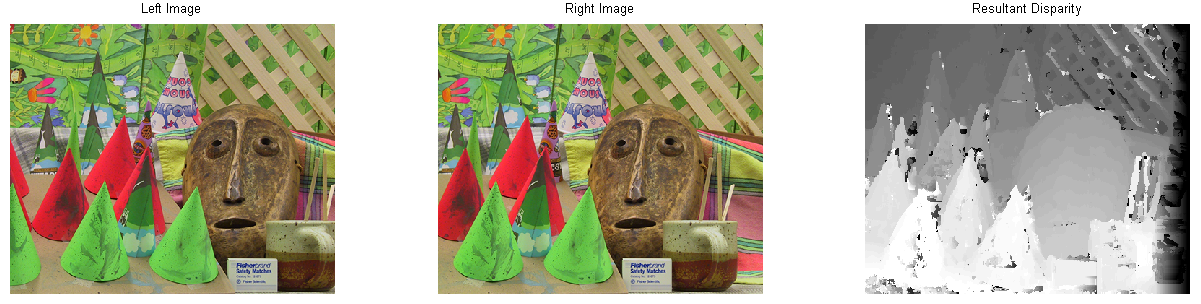
\includegraphics[width=1.2\textwidth]{disparity.png}}
	\caption{Disparity Implementation Output}
	\label{dispMatlabOutput}
\end{figure}

\subsubsection{Verilog Test Bench}
The original Verilog disparity test implementation used closely follows the \textsc{Matlab} disparity algorithm discussed in the previous section. This algorithm is implemented using a finite state machine with five states, as shown in Figure \ref{disparityTestImp} below. In order to maintain simplicity, the test algorithm has been implemented to operate on the 20x7 pixel test images shown in Figure \ref{disparityTestImg}. The search range and block size for this module have been defined as 15 pixels and 5x5 pixels, respectively. By default, the disparity module will remain in an idle state until an external enable signal is toggled high using a button input. This will cause the finite state machine to advance to its READ state, and image data for the left and right camera images will be read in from the stereo camera breakout board. After image data has been received, the state machine will then advance to a cyclical set of states used for iterating through each image and calculating disparity. 
\par
\begin{figure}[H]
	\centerline{
\includegraphics[width=0.75\textwidth]{disp_tb/testImages.png}}
	\caption{Disparity Test Images}
	\label{disparityTestImg}
\end{figure}
The disparity module will begin by isolating the template and search blocks from the right and left image data in the finite state machine's separation state. Next, the state machine will advance to its SAD state, and will calculate the sum of absolute differences between the template and search block. This value is placed in a vector that matches the length of the search range. If the vector hasn't been completely filled, indicating that there are more search blocks to compare to the template, the state machine will revert back to the separate state, isolating a new search block from the right camera image. When the SAD vector is full, the state machine will advance to its finalization state. 
\par
\begin{figure}[H]
	\centerline{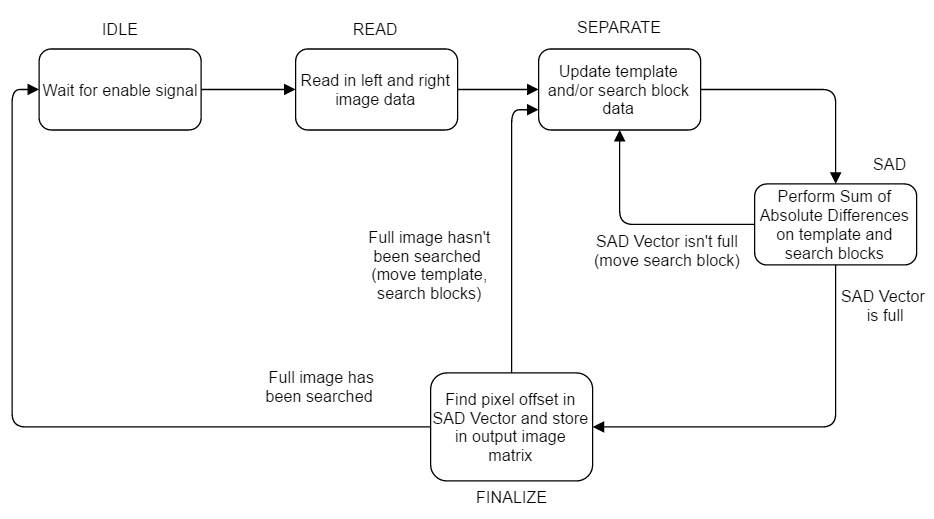
\includegraphics[width=1.0\textwidth]{looping_disparity.png}}
	\caption{Disparity Test Implementation}
	\label{disparityTestImp}
\end{figure}
\par
The finalization state is used to search through the SAD vector for the lowest value. The index of this value within the SAD vector in reference to the template block location is used to create a disparity value for the given template block location. This value is then converted to a distance using Equation \ref{disp2dist}, and is stored in the output image location. If the output image hasn't been fully populated with distance values, the state machine will then revert back to the separate state. Otherwise, the state machine will advance to its idle state, and the resulting disparity image can be read for output. 
\par
This module was initially tested using a Verilog Test Bench, and was then tested using camera image data and a VGA display controller module, allowing for real-time verification of the algorithm's effectiveness. After testing the initial disparity algorithm, several modifications were made to increase the overall speed and efficiency of the disparity module. 
\subsubsection{Test Bench Results}
The READ state of the disparity state machine was first analyzed using the Verilog Test Bench, and the these test results are shown in Figure \ref{disparityImgRead} below. The state machine is shown transitioning from IDLE (0) to READ (1) in the beginning of the timing diagram, as shown by output indicator \texttt{state\_LED}. After transitioning to its READ state, the disparity module reads in each image horizontally from left to right, as dictated by \texttt{buffer\_href} and \texttt{buffer\_vref}. The left camera image is read first, and output \texttt{image\_sel} is then toggled to signal a second read sequence from the right camera image buffer. During each rising clock cycle, input \texttt{image\_data} is stored in an internal BRAM module for the associated camera's image data, with the write address based on the current value of \texttt{buffer\_href} and \texttt{buffer\_vref}. 

\par
\begin{figure}[H]
	\centerline{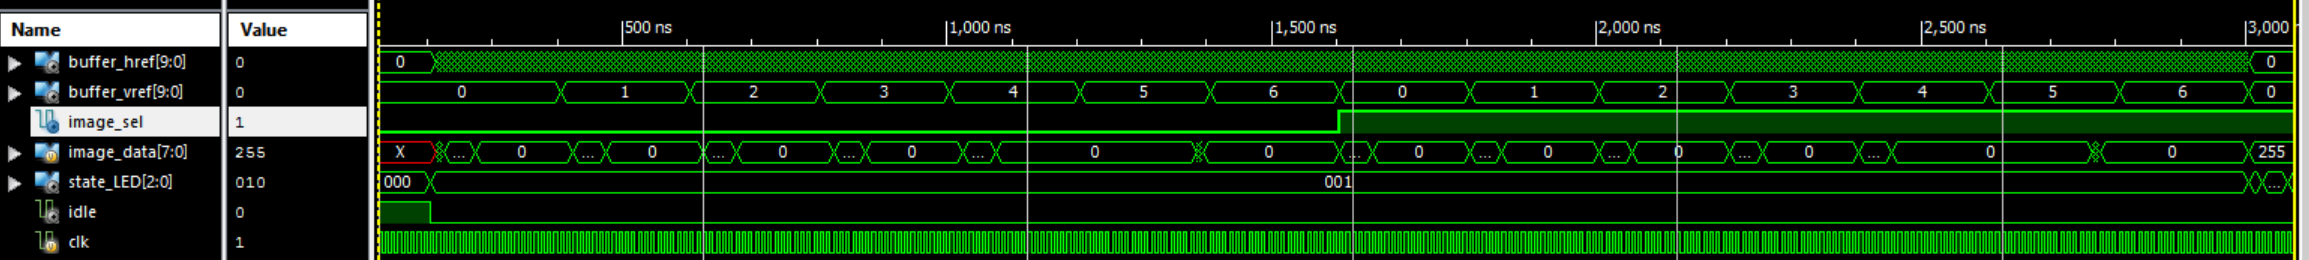
\includegraphics[width=1.25\textwidth]{disp_tb/read_bothimages.png}}
	\caption{Image Read Sequence}
	\label{disparityImgRead}
\end{figure}
\par

After the state machine finishes reading both images into local BRAM on the Zynq7 processor, it will iterate through the SEPARATE (2) and SAD (3) states until an entire search range of search blocks have been compared to the given template block. After the search range has been traversed, the state machine will advance to its FINALIZE (4) state to find the disparity value for the given search and place the value in the output buffer. Figure \ref{disparityVector} shows an example of this process, where a template block set by pixel row bounds \texttt{minr} and \texttt{maxr} and pixel column bounds \texttt{t\_minc} and \texttt{t\_maxc} is compared to 15 individual search blocks set by row bounds \texttt{minr} and \texttt{maxr} and column bounds \texttt{b\_minc} and \texttt{b\_maxc}.
\par
\begin{figure}[H]
	\centerline{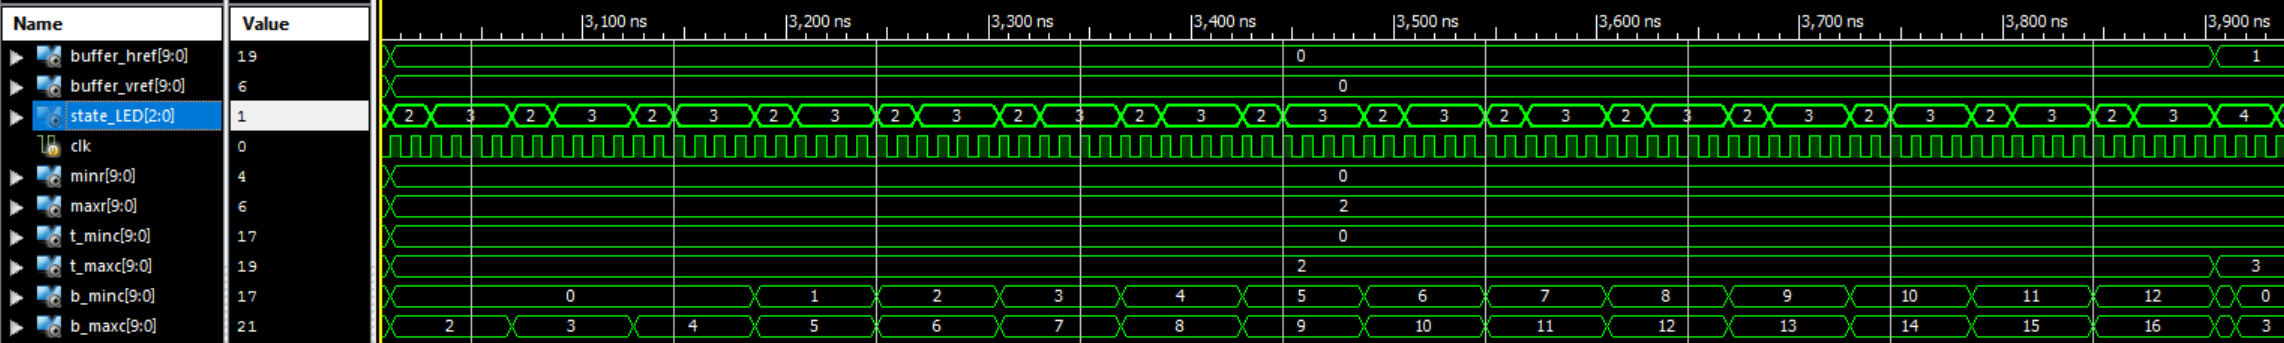
\includegraphics[width=1.25\textwidth]{disp_tb/disparity_vector.png}}
	\caption{Disparity Search Vector}
	\label{disparityVector}
\end{figure}
\par
Note that in the case of the disparity search shown in Figure \ref{disparityVector} above, a disparity value is being calculated for the pixel location (0,0), or the top left corner of the image, as defined by \texttt{buffer\_href} and \texttt{buffer\_vref}.
\par
After each disparity search is completed, the state machine will advance from the FINALIZE state to the SEPARATE state to isolate a new template block and search block. Internal counters for horizontal and vertical pixel location of the disparity search are also updated at this point, triggering an update of the template and search block parameters, as well as the number of blocks to analyze in the current disparity search. This number decreases as the template block gets closer to the right side of the image, since the search range will eventually exceed the distance from the template block to the width (right edge) of the image. An example of multiple disparity searches across one horizontal line of pixels in the top row of the 20x7 test image is shown below in Figure \ref{disparityHorizSearch}. In the case of this example, \texttt{numBlocks} represents the number of blocks to include in the current disparity search. Since the width of the image is 20px and the search range is set to 15px, \texttt{numBlocks} begins to decrease after the 4th disparity search is performed, as shown below.
\par
\begin{figure}[H]
	\centerline{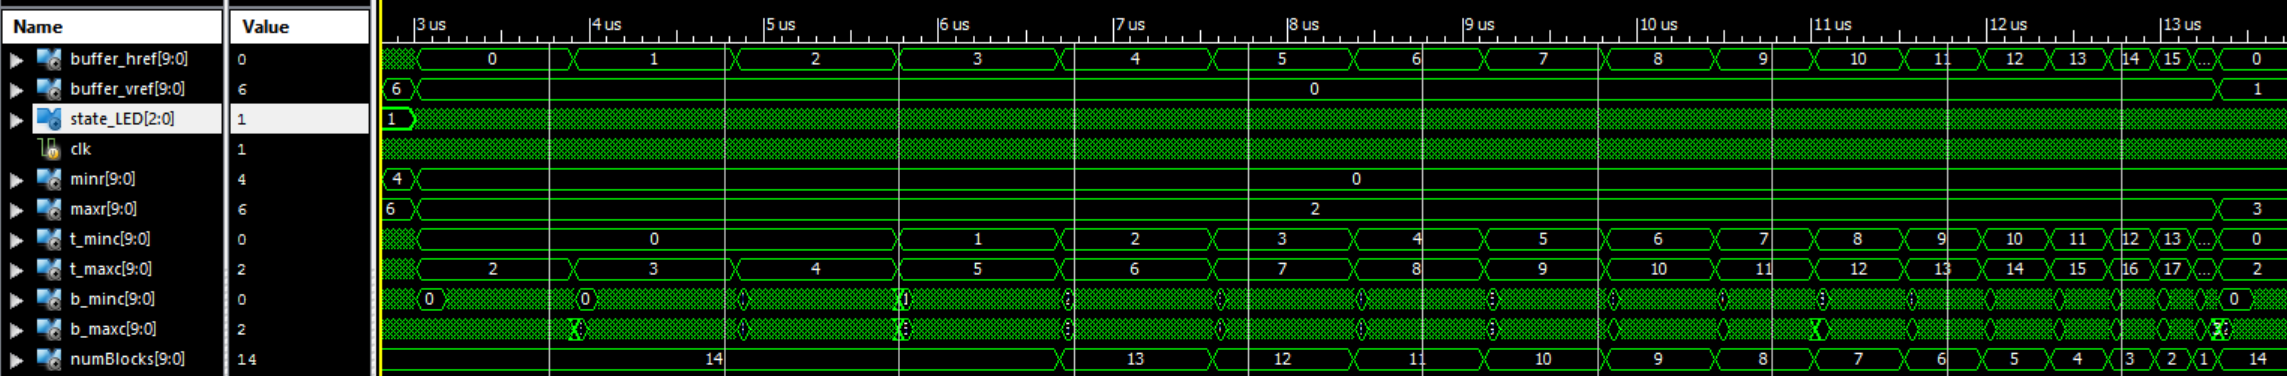
\includegraphics[width=1.25\textwidth]{disp_tb/disparity_fullPixelRow.png}}
	\caption{Horizontal Pixel Row Search}
	\label{disparityHorizSearch}
\end{figure}
\par
After an entire horizontal row of pixels has been analyzed by the disparity algorithm, the vertical location of the template block is increased, and the overall process is repeated continuously until the entire image has been analyzed. An example of a disparity search through the entire 20x7 image is shown below in Figure \ref{disparityFullSearch}.
\par
\begin{figure}[H]
	\centerline{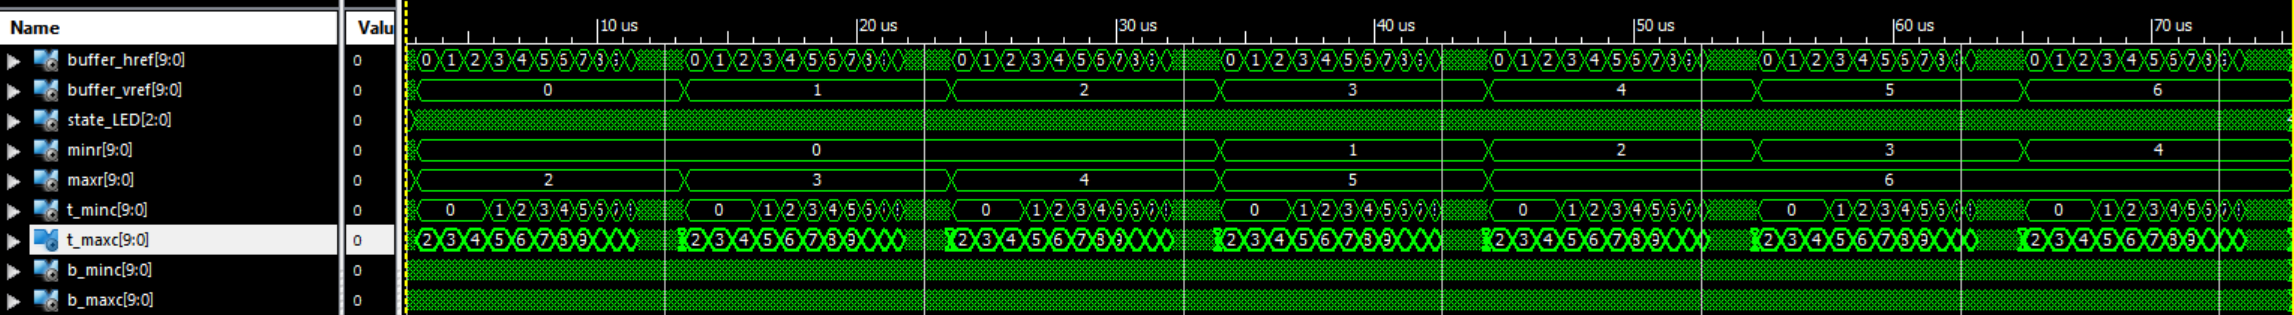
\includegraphics[width=1.25\textwidth]{disp_tb/full_disparity.png}}
	\caption{Full Image Search}
	\label{disparityFullSearch}
\end{figure}
\par
The output disparity image of the test analyzed above is shown below in Figure \ref{disparityTestResults}. Note that the artifacts in the resultant image are due to the fact that a 5x5 template and search block set is being used on a 20x7 image, making it impossible to avoid the block contained in the upper left corner of the search image. The direction of artifacts around the block in the lower right corner of each image are a function of the search direction, since the search blocks descend downwards and to the left.
\par
\begin{figure}[H]
	\centerline{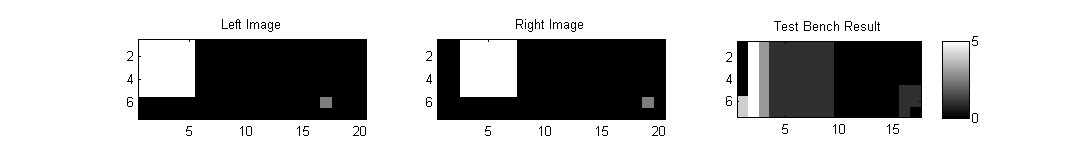
\includegraphics[width=1.0\textwidth]{disp_tb/result_gray.png}}
	\caption{Disparity Test Results}
	\label{disparityTestResults}
\end{figure}
\par
After the disparity module was deemed working on the 20x7 test image, further testing on image data was performed. Through some simple modifications to the Test Bench and a  \textsc{Matlab} script for converting image data to a format recognizable by the Verilog Test Bench's \texttt{\$readmemb} command. Using these converted images, it was then possible to compare the Verilog disparity implementation's results to those of the \textsc{Matlab} implementation. Note that due to limitations in computer memory, the disparity search range and block sizes capable of being processed by the Verilog Test Bench were limited to 15 pixels and 5x5 pixels, respectively. 
\par
Figure \ref{disparityVerilogvsMatlab} below contains a comparison between the test bench and \textsc{Matlab} results for a disparity search on the "cones" test image set. Note that the outputs from the \textsc{Matlab} and Verilog disparity search algorithms are noticeably close in comparison, as well as in pixel intensity. Losses in the the output of the Verilog disparity algorithm are likely due to the fact that all operations are performed using integers rather than floating point values.
\par
\begin{figure}[H] 
         \begin{subfigure}[h]{0.5\textwidth}
              \centerline{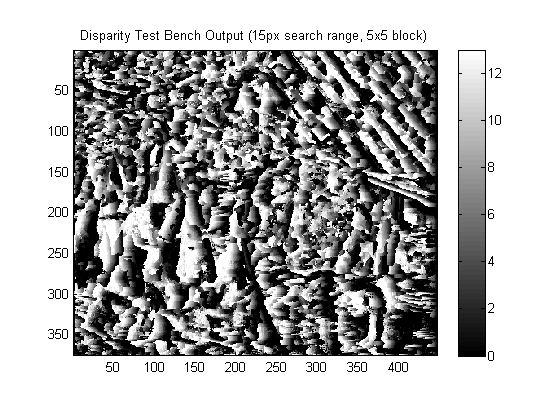
\includegraphics[width=1.1\textwidth]{disp_tb/tb_cones.png}}
             \caption{Test Bench Result}
         \end{subfigure}
         \begin{subfigure}[h]{0.5\textwidth}
             \centerline{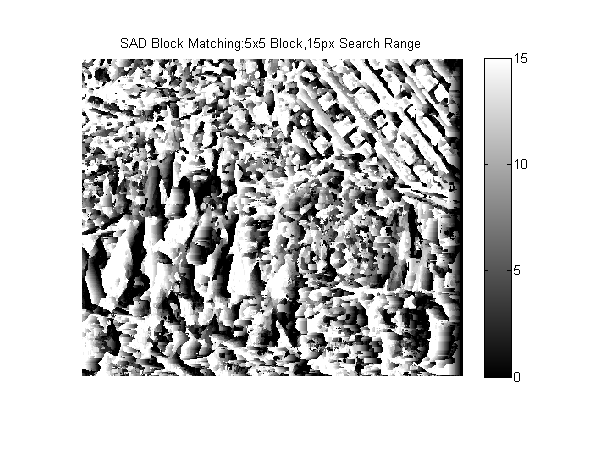
\includegraphics[width=1.1\textwidth]{disp_tb/MATLAB_conesDSP.png}}
             \caption{\textsc{Matlab} Result}
         \end{subfigure}
\caption{\textsc{Matlab} vs. Verilog Test Bench Results}
\label{disparityVerilogvsMatlab}
\end{figure}


\subsubsection{Final Implementation}
In order to increase the speed of the disparity algorithm's output, several portions of the original disparity Verilog module used in the previous section were modified to increase parallelization and decrease the overall latency associated with various calculations. Most of this parallelization was based around taking the 2D memory arrays used for storing the template and search blocks, and breaking said arrays into individual vectors. For example, instead of having a 7x7 memory array for storing one "block" of pixels, the block is broken into seven separate 1x7 vectors that can be operated on individually. This parallelization decreases the overall latency of the system by making it so that there is less time spent waiting to read from individual addresses within memory arrays. An overall block diagram of the more parallel disparity implementation is shown in Figure \ref{disparityFinalImp} below. 
\par
\begin{figure}[H]
	\centerline{\includegraphics[width=1.2\textwidth]{Disparity_Algorithm.png}}
	\caption{Disparity Final Implementation}
	\label{disparityFinalImp}
\end{figure}
\par
The overall state machine used to create the final disparity implementation still follows the same next state logic as that of the original implementation, shown in Figure \ref{disparityTestImp}. Advances in speed of the overall algorithm are therefore mostly associated with parallel calculations during the computation of the Sum of Absolute Differences. As discussed in Section \ref{dataman}, the left and right search images passed to the disparity algorithm are also windowed to $0.6*VGA$ resolution. 
\par
In order to verify the output of the hardware disparity implementation, a VGA display driver is used to display the disparity algorithm's output in real time, as shown in Figure \ref{disparityFin}. With the successful implementation of this output mode, it was then possible to concentrate on combining the disparity and camera controller modules into a final design that incorporated the IMU and Rangefinder modules.
\par
\begin{figure}[H] 
	\begin{subfigure}{0.5\textwidth}
	\centering
		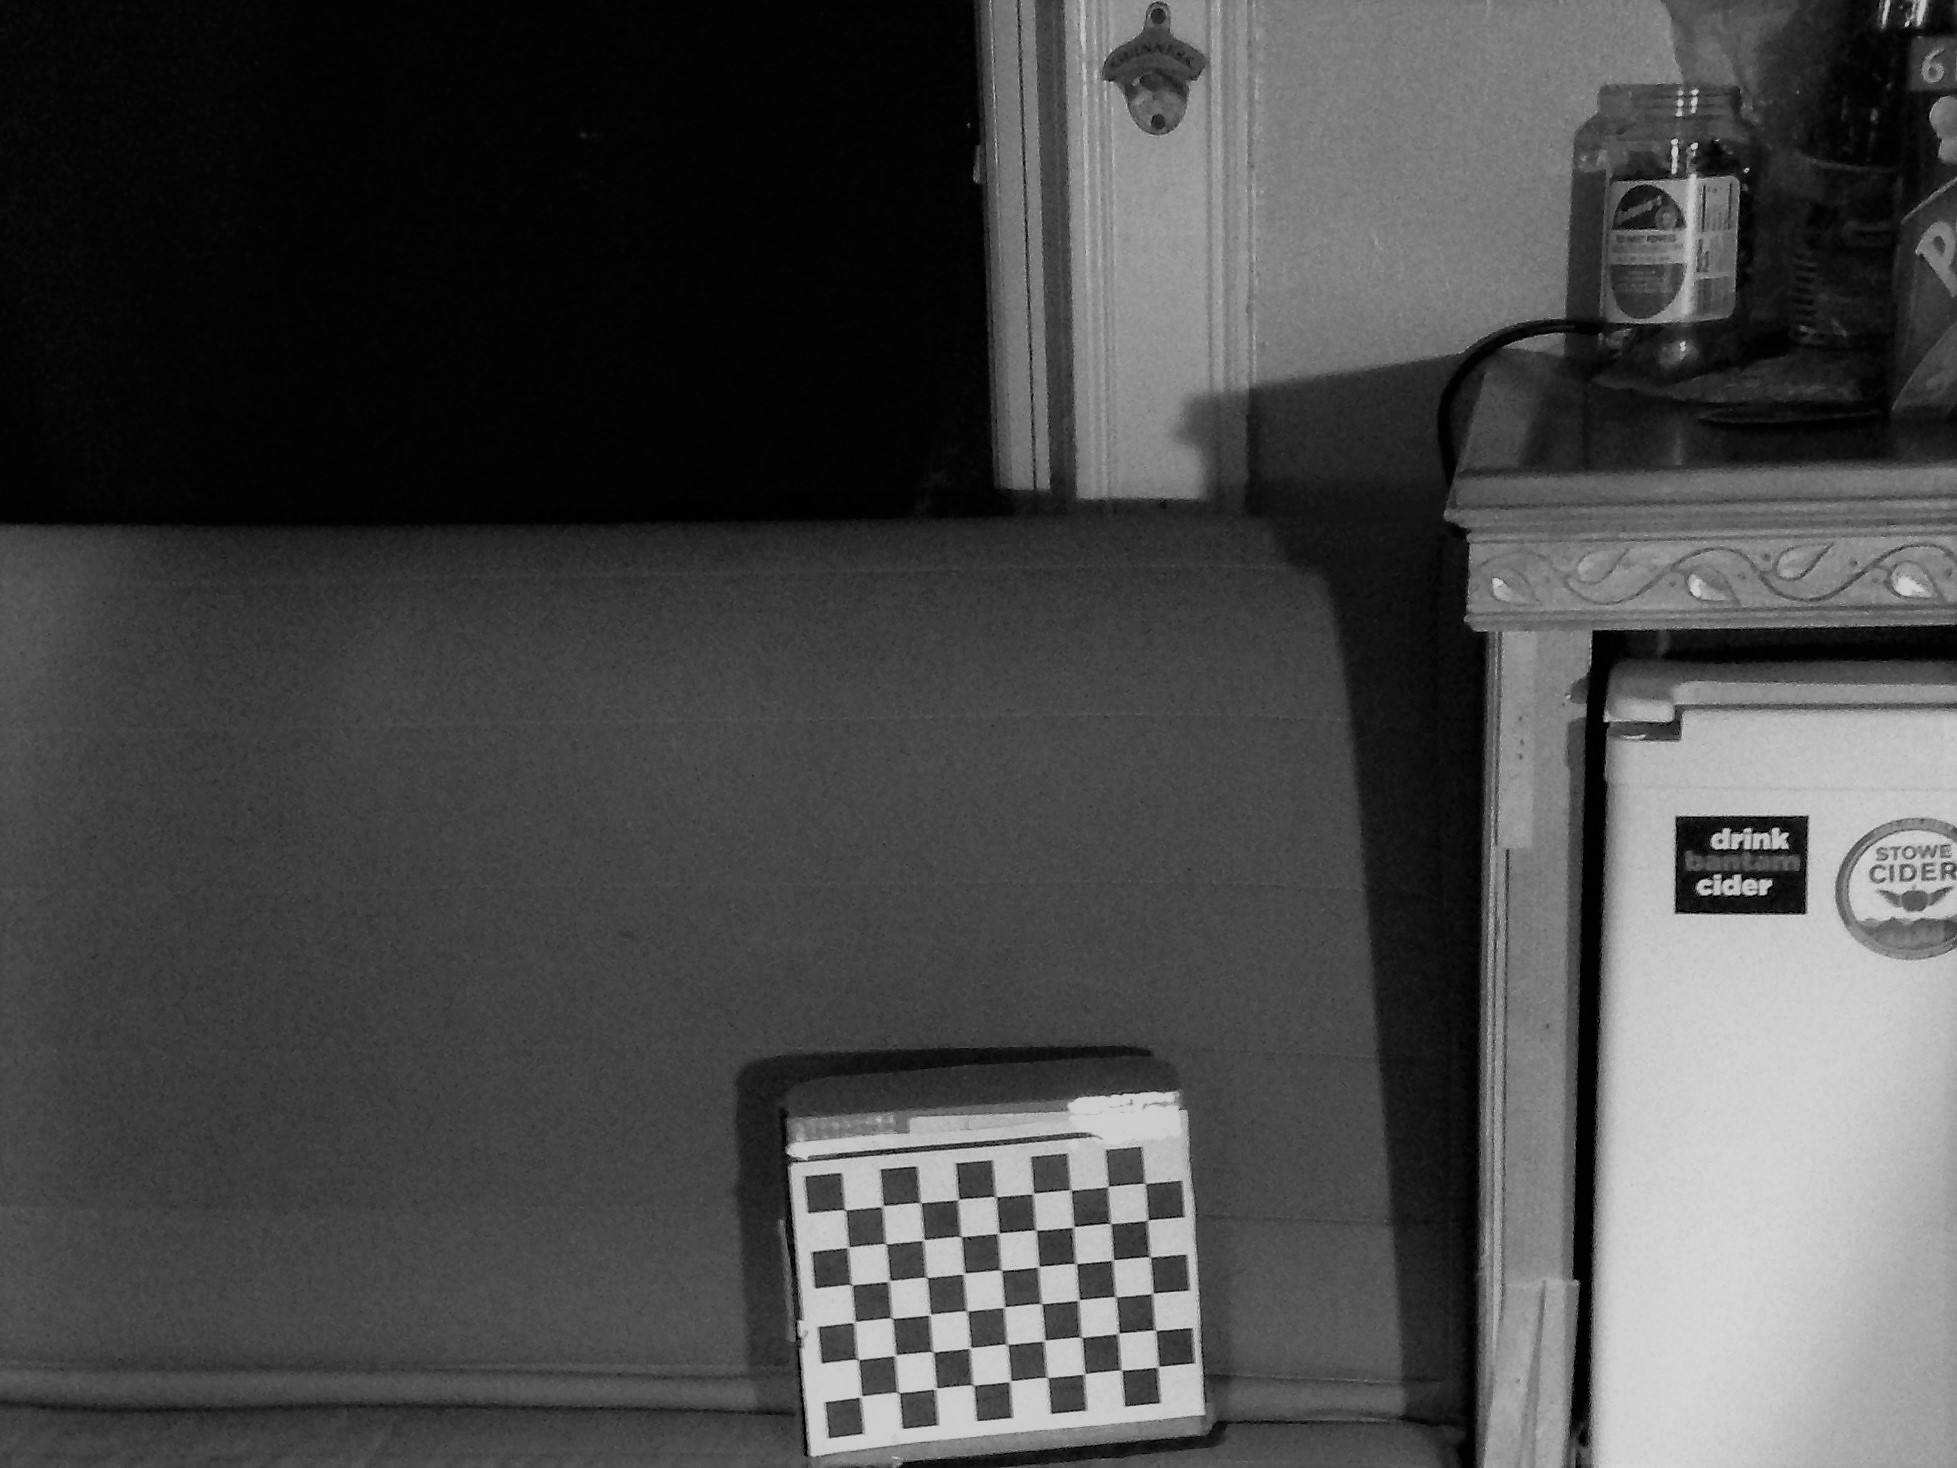
\includegraphics[width=0.8\linewidth]{disparity_rtView.JPG}
		\caption{Device View}
	\end{subfigure}
	\begin{subfigure}{0.5\textwidth}
	\centering
		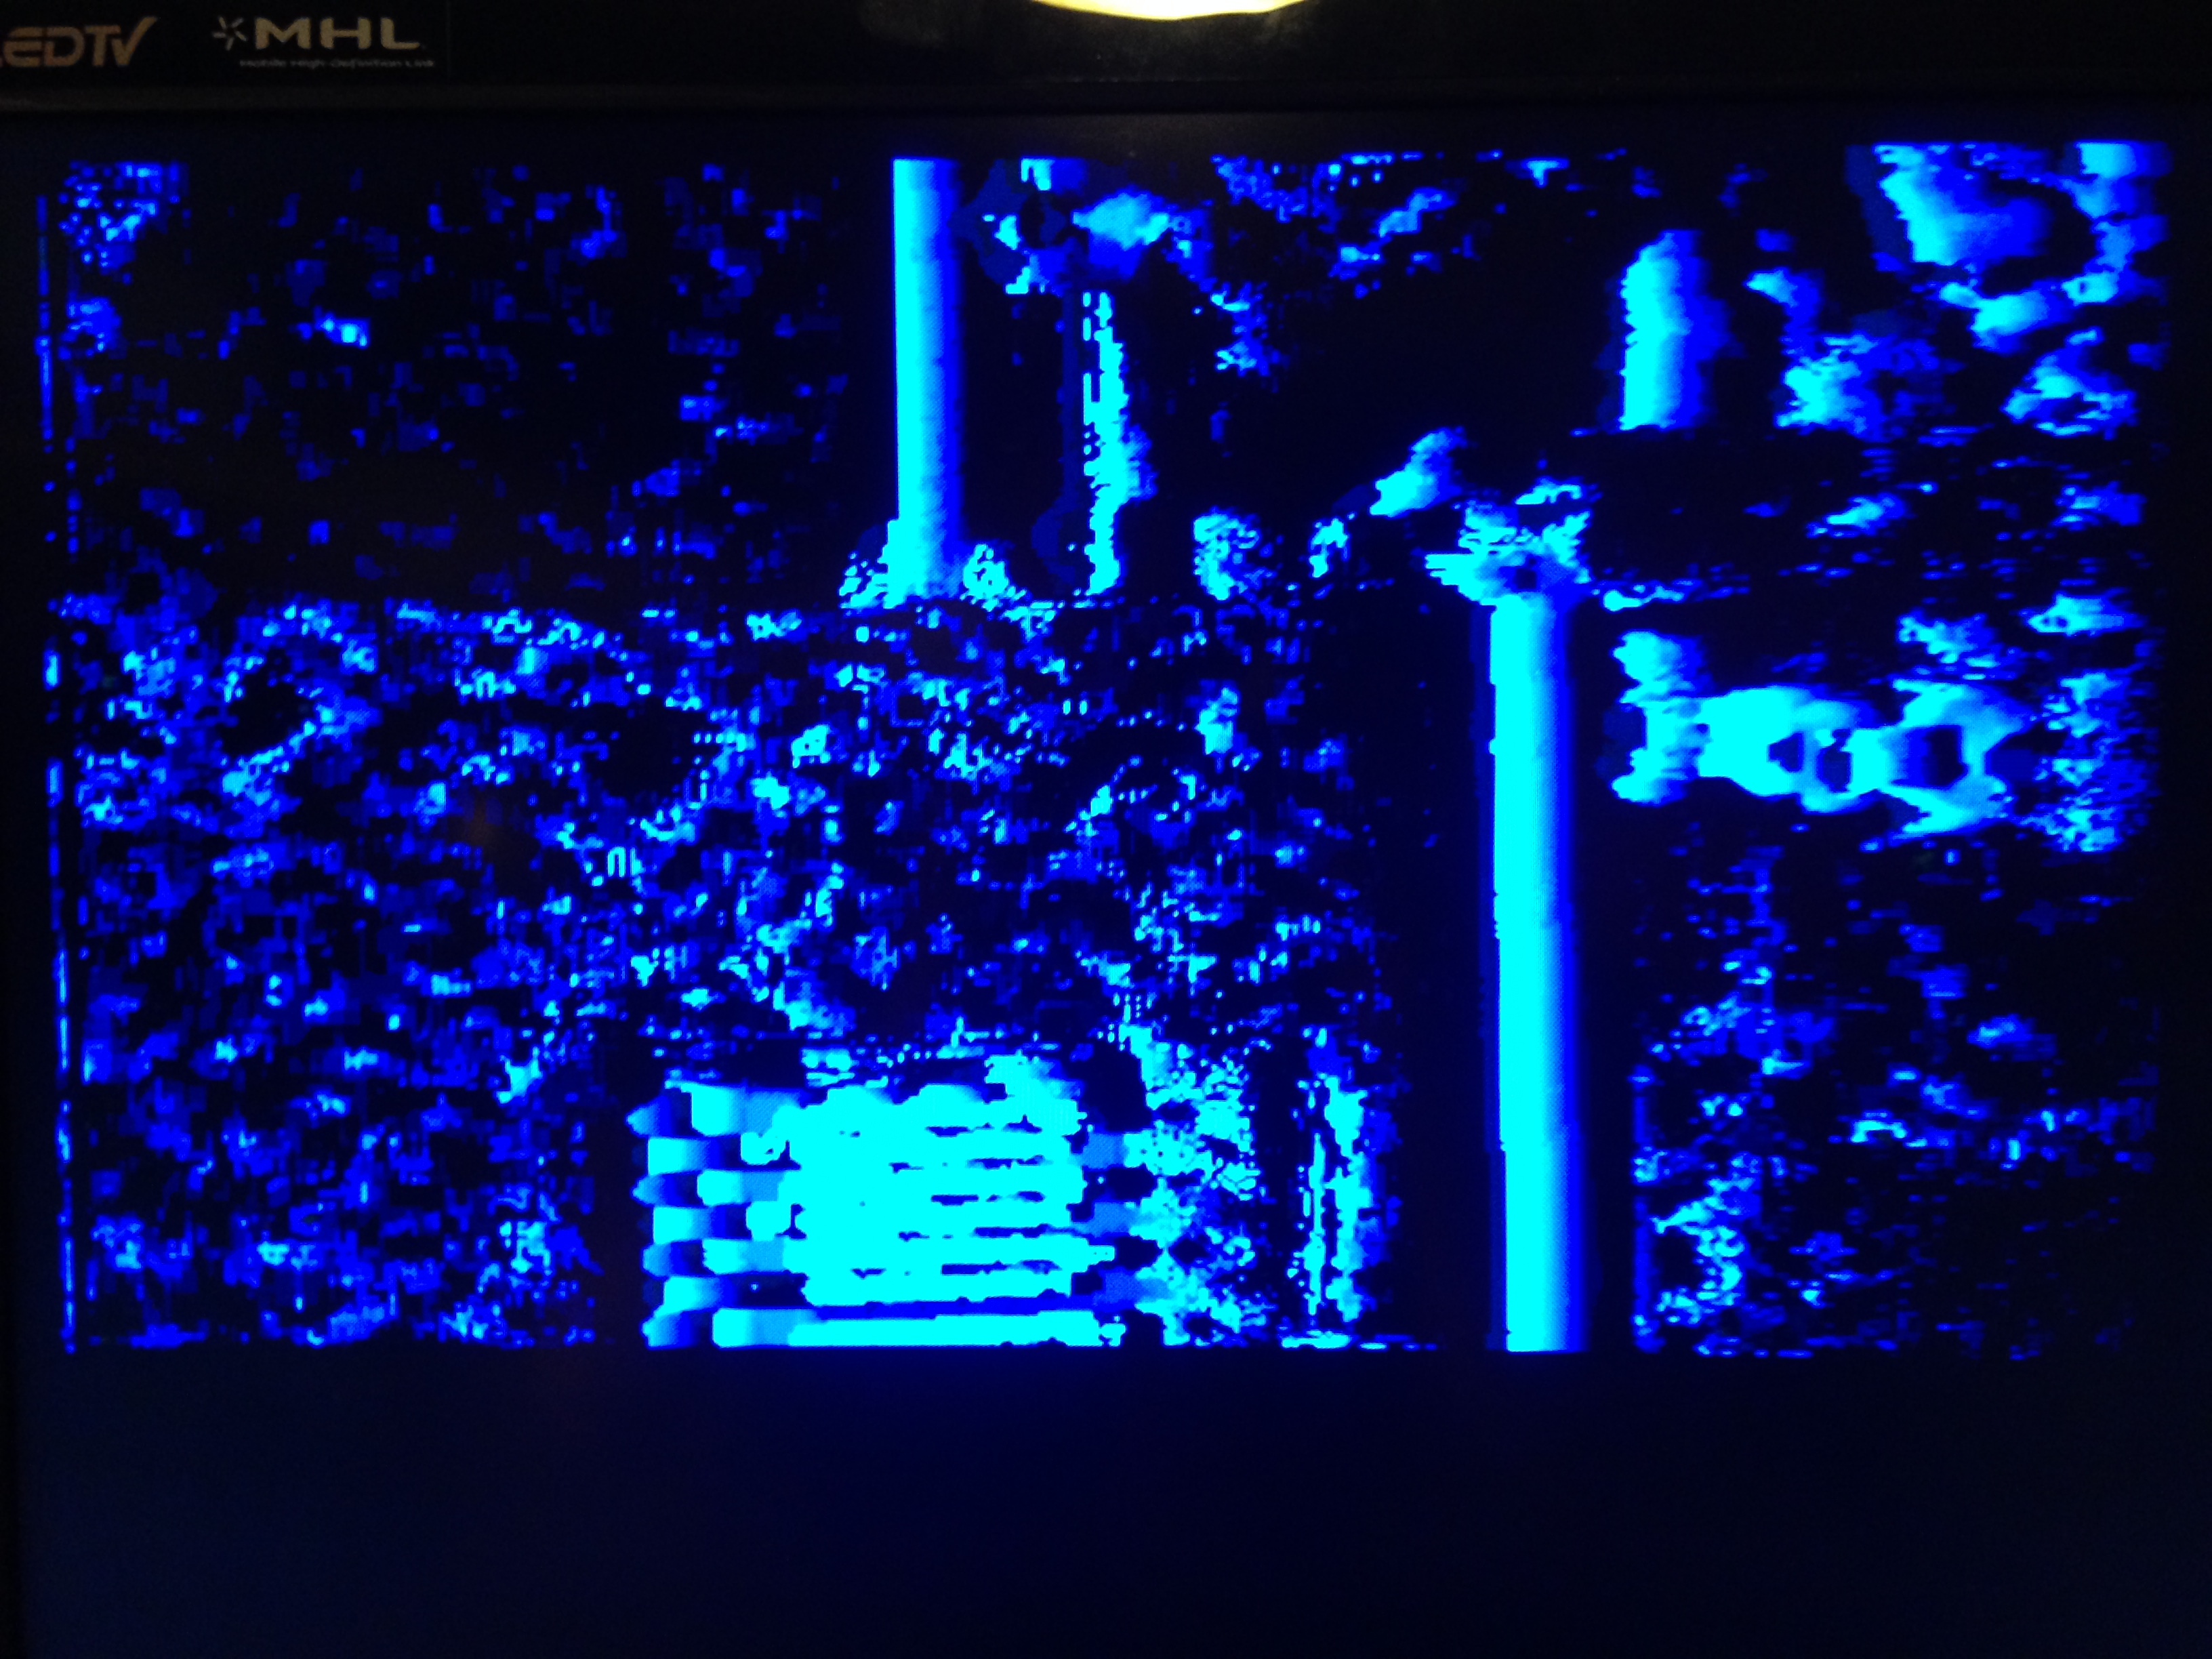
\includegraphics[width=0.8\linewidth]{disparity_rt.JPG}
		\caption{Resultant Disparity}
	\end{subfigure}
	\caption{Disparity Algorithm Output}
	\label{disparityFin}
\end{figure}